\section{System's Perspective}
\subsection{Design and Architecture}
\textcolor{red}{Design and architecture of your ITU-MiniTwit systems. All dependencies of your ITU-MiniTwit systems on all levels of abstraction and development stages.}
\subsubsection*{Overview of System Design}
\subsubsection*{Architecture Diagram}
\subsection{Technologies and tools}
\textcolor{red}{That is, list and briefly describe all technologies and tools you applied and depend on.}
\subsubsection*{List of Technologies and Tools Utilized}
\begin{multicols}{2}
    \begin{itemize}
        \item \textbf{Go}: A statically typed, compiled programming often used for backend development.
        \item \textbf{Go/Gorilla}: A toolkit for Golang, that provides packages for building web applications. Used for routing and session management.
        \item \textbf{SQLite}: A lightweight SQL database engine that is ideal for embedded database applications. Used in initial setup and for testing.
        \item \textbf{Docker}: A platform for shipping and running applications, ensuring consistency across different environments. Containerization is used deliberately throughout our system and in delivery.
        \item \textbf{Vagrant}: A tool for building and managing virtualized development environments. Used initially for VM instantiating.
        \item \textbf{DigitalOcean}: A cloud infrastructure provider offering scalable compute and storage solutions. Used for deploying and managing the application and database.
        \item \textbf{CircleCI}: A continuous integration and delivery platform that automates the build, test and deployment processes of our project.
        \item \textbf{CodeClimate}: A platform that provides code review, offering insights into code quality, maintainability and test coverage, helping us ensure high standards and to improve code health.
        \item \textbf{Prometheus}: An open-source monitoring toolkit used for monitoring metrics in our cloud environments.
        \item \textbf{Grafana}: An open-source analytics and monitoring platform that integrates various data sources to visualize our data and metrics.
        \item \textbf{PostgreSQL}: A open-source object-relational database system, known for extensibility and speed. Used after the transition from SQLite managed by DigitalOcean.
        \item \textbf{Promtail}: An agent that ships log file to Loki and part of the Grafana logging stack. Used for gathering logs.
        \item \textbf{Loki}: A log aggregation system designed to be scalable. Used with Grafana for log querying and visualization.
        \item \textbf{Nginx}: A high-performance web server and reverse proxy server. Used for load balancing.
        \item \textbf{CertBot}: A open-source tool for automatically using Let's Encrypt certificates to enable HTTPS on web servers.
        \item \textbf{Terraform}: An infrastrcucture as code tool that allows users to define and provision data center infrastructure using a high-level configuration language. %maybe
    \end{itemize}
\end{multicols}



\subsection{Subsystem interactions}
\textcolor{red}{Important interactions of subsystems.
For example, via an illustrative UML Sequence diagram that shows the flow of information through your system from user request in the browser, over all subsystems, hitting the database, and a response that is returned to the user.
Similarly, another illustrative sequence diagram that shows how requests from the simulator traverse your system.}
\begin{figure}[H]
    \centering
    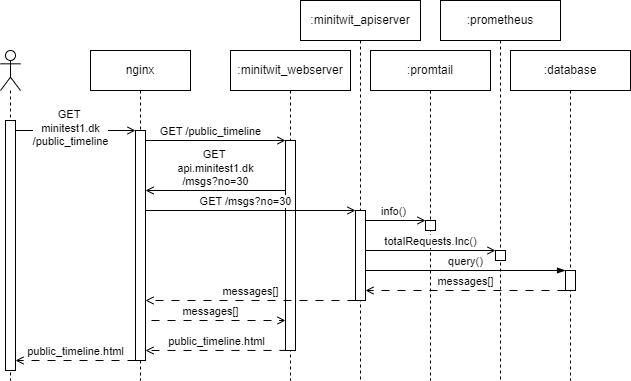
\includegraphics[width=0.8\textwidth]{images/sequence.png}
    \caption{Minitwit\_Dashboard - API Monitoring}
    \label{fig:monitor_good}
\end{figure}
\subsection{Current state}
\textcolor{red}{Describe the current state of your systems, for example using results of static analysis and quality assessments.}
At the time of writing, 

\subsection{Technology choices}%should maybe just be in text when relevant
\textcolor{red}{MSc should argue for the choice of technologies and decisions for at least all cases for which we asked you to do so in the tasks at the end of each session.}
Our initial choice of language for refactoring ITU-MiniTwit was based on a detailed feature mapping of the system and a comparison of programming languages (see Appendix \ref{app:programming_language_choice}). 
This analysis led us to initially select Crystal/Kemal. However, we soon discovered that Kemal's documentation was insufficient, making it challenging to work with. Consequently, we switched to Golang, which offered similar features but had much more comprehensive documentation.